\section{Datasets}
\label{sec:datasets}

Data for this report comes from different members of the consortium. The first dataset, is the one anticipated in the previous deliverable on data assimilation. It is generated by Giovanni Grassi (DC6) at CORIA and descibes a Hydrogen-Ammonia blend. This data contains different boundry conditions, making it suitable for pattern identification within the same phoenomena across different scenatios. Moreover the study of the behaviour of combustion of Hydrogen-Ammonia blends is extremely important in the scope of reducing NOx emission, one of the main objectives of the overall project.     
The second dataset is generated by Lorenzo Fracino (DC2) at RWTH Aachen and rapresents a Mehtane-Hydrogen mixing layer.  
\subsection{NH$_3$/H$_2$ non-premixed mixing layer}
\label{sec:DATA_CORIA}

This dataset consists of direct numerical simulations (DNS) of a two-dimensional non-premixed ammonia-hydrogen-air reacting mixing layer. It is generated by DCGIOVANNI at CORIA using the structured mesh reactive flow solver SiTCom-B \cite{sitcomb}. The configuration represents a splitter-plate stabilized flame in which a cold fuel stream and a hot air stream interact across a shear layer, representative of conditions encountered in practical burners. 


The lower stream consists of a NH$_3$/H$_2$ fuel blend (with 15\% H$_2$ by volume) at ambient temperature (300~K) with a mean velocity of 15~m~s$^{-1}$, while the upper stream consists of preheated air with a mean velocity of 39.6~m~s$^{-1}$. A cold wall maintained at 600~K is imposed at the top boundary, and a symmetry condition is applied at the bottom. Homogeneous velocity fluctuations of 10\% are prescribed at both inlets. The computational domain measures $12 \times 1$~cm and is discretized on a uniform grid of $2400 \times 200$ cells with a resolution of 50~$\mu$m. 

\FloatBarrier
\begin{figure}[htbp]
    \centering
    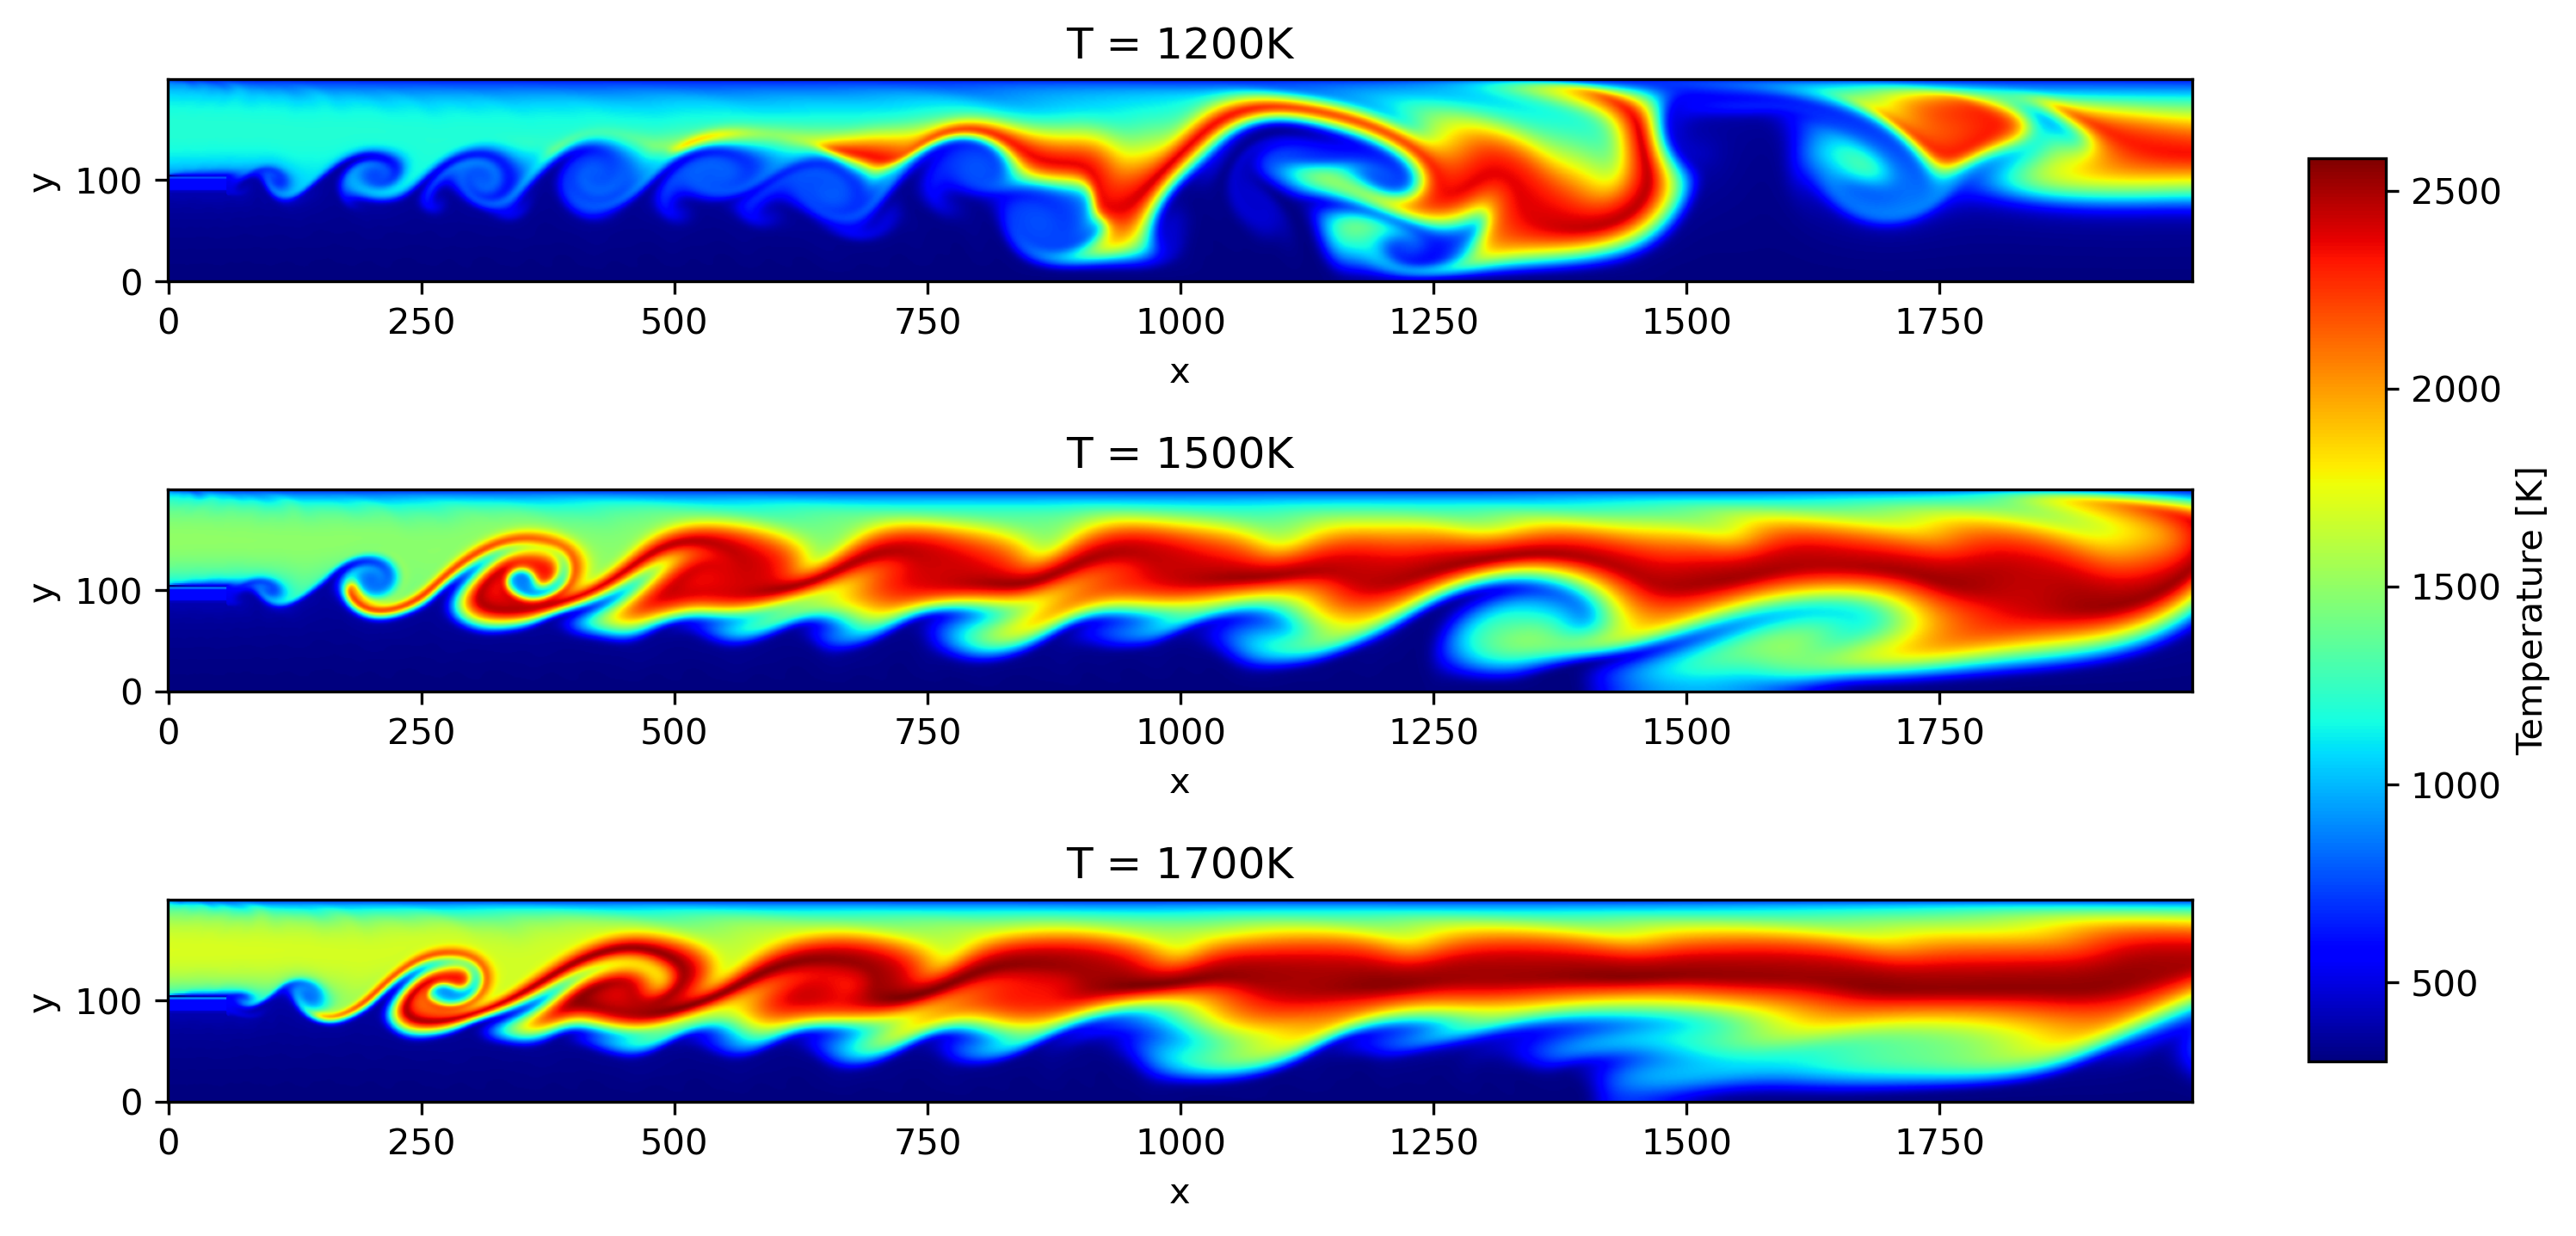
\includegraphics[width=0.85\textwidth]{../IMAGES/DATASETS/coria_3snap.png}
    \caption{Three representative snapshots of the temperature field from the NH$_3$/H$_2$ non-premixed reacting mixing layer DNS, illustrating the spatial evolution of the flame and mixing structures at different instants.}
    \label{fig:coria_data}
\end{figure}
\FloatBarrier

Three datasets are generated at different air preheat temperatures, namely 1200~K, 1500~K, and 1700~K, to probe the sensitivity of the flame dynamics and species evolution to the inlet thermal boundary condition. The domain geometry, grid resolution, and flow velocities are identical across all three cases. Each snapshot contains 19 reactive scalar fields corresponding to the species of the reduced mechanisms RmAH-1 and RmAH-2 \cite{grassi2025} — namely H$_2$, O$_2$, H$_2$O, H, O, OH, HO$_2$, NH$_3$, NH$_2$, NH, N, NO, NO$_2$, N$_2$O, HNO, NNH, N$_2$H$_2$, N$_2$, and Ar — together with temperature, yielding 20 variables in total. The species analysis presented in this work is conducted exclusively on the 1500~K dataset, which constitutes the reference operating condition for the assessment of the proposed methodologies.
\begin{comment}
    
\subsection{CH$_4$/H$_2$ MILD combustion mixing layer}
\label{sec:DATA_RWTH}

This dataset consists of direct numerical simulations (DNS) of a temporally evolving three-stream mixing layer representative of MILD (Moderate or Intense Low-oxygen Dilution) combustion conditions. It is generated at the Institute for Combustion Technology of RWTH Aachen University using the in-house finite-difference solver CIAO \cite{frascino2025}, which solves the reactive unsteady Navier--Stokes equations in the low-Mach-number limit. The full dataset and its physical analysis are described in detail in \cite{frascino2025}.


The configuration consists of three co-flowing streams: a central cold fuel jet of 25\%~H$_2$/75\%~CH$_4$ (by volume) at $T_\mathrm{fuel} = 300$~K, flanked by two jets of preheated air at $T_\mathrm{air} = 900$~K, which are in turn surrounded by streams of lean hot combustion products at $T_\mathrm{hot} = 1225$~K. The equivalence ratio of the mixture is $\phi = 0.8$. Periodic boundary conditions are imposed in the streamwise ($x$) and spanwise ($z$) directions, while an outlet condition is applied in the cross-stream ($y$) direction. The DNS is initialised from 1D flamelet profiles mapped onto a smooth mixture-fraction field, placing the simulation in a quasi-frozen state that allows the onset of autoignition to be captured. The chemical kinetics are described by a reduced mechanism for lean CH$_4$/H$_2$ combustion comprising 24 species and 251 reactions, derived from the full C3MechV3.3 model \cite{dong2022}.

The dataset comprises four cases obtained by independently varying two Damk\"{o}hler numbers: $Da_\mathrm{HA}$, associated with the hot-products--air mixing process, and $Da_\mathrm{FA}$, associated with fuel--air mixing. High $Da_\mathrm{HA}$ values correspond to high-dilution (HD) conditions characteristic of the MILD regime, while low $Da_\mathrm{HA}$ values correspond to low-dilution (LD), non-MILD conditions. Each dilution condition is combined with a fast ($Da_\mathrm{FA}$ low) or slow ($Da_\mathrm{FA}$ high) fuel--air mixing rate, yielding the four cases HD-FF, HD-SF, LD-FF, and LD-SF. The computational grid contains approximately $1.2 \times 10^9$ cells for the HD cases and $0.7 \times 10^9$ cells for the LD cases, with a minimum of 10 grid points resolved across the OH reaction layers and a ratio $\Delta/\eta < 2$ ensuring that the Kolmogorov scale is well resolved throughout the domain.

\subsubsection*{Filtered DNS}

The data used in the present work is not the raw DNS output but a spatially filtered version of it, obtained by applying a box filter of width $\Delta_f = 8\,\Delta_\mathrm{DNS}$ to the DNS fields, where $\Delta_\mathrm{DNS}$ denotes the local DNS grid spacing. This filtered DNS (fDNS) retains the large-scale coherent structures and the dominant dynamical features of the flow while suppressing the smallest dissipative scales, making the dataset tractable for the tensor-based analysis described in Section~\ref{sec:methods}.

% -------------------------------------------------------
% TODO — ask the data provider (Lorenzo Frascino / RWTH):
%   1. Which of the four cases (HD-FF, HD-SF, LD-FF, LD-SF) are available?
%   2. Confirm filter type: box filter (top-hat) with Delta_f = 8 * Delta_DNS?
%   3. What variables are provided? (temperature + all 24 species, or a subset?)
%   4. Number of snapshots and temporal spacing Delta_t for each case?
% -------------------------------------------------------
\end{comment}

\subsection{ULB hydrogen-fueled flameless furnace}
\label{sec:DATA_ULB}

This dataset consists of computational fluid dynamics simulations of a hydrogen-fueled semi-industrial furnace operating under flameless combustion conditions. The work is conducted by Isacco Faglioni (UPM Madrid), Chiara Novelli (ULB Brussels), and Alessandro Parente (ULB Brussels, BRITE) as part of the CYPHER project. Two main methodological approaches are applied to this dataset: uncertainty quantification using POD/GPR and tensor-based reduced order modeling using HOSVD/GPR.

The furnace is based on the ULB-modified SPRF (Semi-industrial Perfectly stirred Reactor Furnace) configuration, consisting of a cubic combustion chamber (700 × 700 × 700 mm inner dimensions) fired by a bottom-mounted commercial burner with an integrated heat exchanger for air preheating. The fuel injection system features a centrally located nozzle with 8 mm internal diameter, surrounded by a coaxial air jet with variable diameter to adjust entrainment.

\FloatBarrier
\begin{figure}[htbp]
    \centering
    % TODO: Add figure showing the ULB furnace geometry and temperature field
    % \includegraphics[width=0.85\textwidth]{../IMAGES/DATASETS/ulb_furnace.png}
    \caption{[PLACEHOLDER] Cross-section of the ULB flameless furnace showing the geometry and qualitative sketch of the mean temperature field.}
    \label{fig:ulb_data}
\end{figure}
\FloatBarrier

\subsubsection*{Uncertainty quantification study}

The first application focuses on uncertainty quantification using POD/GPR methodology to assess parametric uncertainty propagation in 2D RANS simulations. The analysis considers 9 uncertain input parameters: 3 kinetic rate constants (reactions R3, R5, R16 of H$_2$ core mechanism), 3 turbulence model parameters (realizable $k-\varepsilon$ constants $C_{2\varepsilon}$, $\sigma_k$, $\sigma_\varepsilon$), 1 combustion model parameter (PaSR mixing constant $C_{mix}$), and 2 operational parameters (fuel and air mass flow rates).

Operating conditions include 100\% H$_2$ fuel, 15 kW nominal power, 5.1 kW cooling power, equivalence ratio $\phi = 0.8$, and 16 mm air inlet diameter. The dataset comprises 128 RANS simulations using Latin Hypercube Sampling, with temperature and species mass fractions (H$_2$O, OH) monitored across 48 probe locations. The sensitivity analysis reveals that turbulence parameter $C_{2\varepsilon}$ and combustion constant $C_{mix}$ dominate the response variance (91.4\% total contribution), with air mass flow rate contributing significantly in recirculation regions.

\subsubsection*{Tensor-based reduced order modeling}

The second application develops an alternative approach using High Order Singular Value Decomposition (HOSVD) combined with Gaussian Process Regression to create digital twins for flameless combustion. The data is structured as a 5-way tensor $\mathcal{T} \in \mathbb{R}^{N_\phi \times N_{H_2} \times N_p \times N_{feat} \times N_{cells}}$ representing 20 operating conditions across equivalence ratio $\phi \in \{1.1, 1.2, 1.3, 1.4, 1.6\}$, H$_2$ blending $\{0.0, 0.3\}$ vol\%, and pressure $\{1, 2\}$ atm.

The HOSVD+GPR methodology decomposes the tensor into a core and factor matrices, interpolates only along the equivalence ratio dimension while freezing other factors, and reconstructs fields for unseen conditions. This approach outperforms classical POD+GPR on all 10 thermochemical variables, demonstrating superior data efficiency in scarce training regimes. The multilinear decomposition preserves physical interpretability and maintains consistency across parameter dimensions, making it particularly suitable for parametric interpolation in reactive flow digital twins.

\subsubsection*{Results and Discussion}

\paragraph{Uncertainty Quantification Results}

% TODO: Add description of POD/GPR model validation
% TODO: Discuss k-fold cross validation results

\FloatBarrier
\begin{figure}[htbp]
    \centering
    % TODO: Add figure showing POD/GPR validation results
    % \includegraphics[width=0.85\textwidth]{../IMAGES/RESULTS/ulb_pod_validation.png}
    \caption{[PLACEHOLDER] POD/GPR model validation results showing temperature parity plot and cross-validation metrics.}
    \label{fig:ulb_pod_validation}
\end{figure}
\FloatBarrier

% TODO: Describe uncertainty propagation in temperature predictions
% TODO: Discuss variance bands and experimental comparison

\FloatBarrier
\begin{figure}[htbp]
    \centering
    % TODO: Add figure showing uncertainty propagation
    % \includegraphics[width=0.85\textwidth]{../IMAGES/RESULTS/ulb_uncertainty_propagation.png}
    \caption{[PLACEHOLDER] Uncertainty propagation for temperature predictions along different axial locations showing 25th-75th percentiles and experimental measurements.}
    \label{fig:ulb_uncertainty}
\end{figure}
\FloatBarrier

% TODO: Present global sensitivity analysis results

\FloatBarrier
\begin{figure}[htbp]
    \centering
    % TODO: Add figure showing Sobol indices
    % \includegraphics[width=0.85\textwidth]{../IMAGES/RESULTS/ulb_sobol_indices.png}
    \caption{[PLACEHOLDER] Total order Sobol indices of the most impactful parameters at probe locations in the ULB furnace.}
    \label{fig:ulb_sobol}
\end{figure}
\FloatBarrier

\paragraph{Tensor-based Model Performance}

% TODO: Describe HOSVD+GPR vs POD+GPR comparison
% TODO: Discuss superior performance across all thermochemical variables

\FloatBarrier
\begin{figure}[htbp]
    \centering
    % TODO: Add figure showing NRMSE comparison
    % \includegraphics[width=0.85\textwidth]{../IMAGES/RESULTS/ulb_nrmse_comparison.png}
    \caption{[PLACEHOLDER] NRMSE comparison between HOSVD+GPR and POD+GPR across all thermochemical variables.}
    \label{fig:ulb_nrmse}
\end{figure}
\FloatBarrier

% TODO: Show temperature field reconstruction results

\FloatBarrier
\begin{figure}[htbp]
    \centering
    % TODO: Add figure showing temperature field reconstruction
    % \includegraphics[width=0.85\textwidth]{../IMAGES/RESULTS/ulb_temperature_reconstruction.png}
    \caption{[PLACEHOLDER] Temperature field reconstruction for unseen condition. Left: CFD reference. Center: HOSVD+GPR. Right: POD+GPR.}
    \label{fig:ulb_temp_reconstruction}
\end{figure}
\FloatBarrier

\paragraph{Discussion}

% TODO: Discuss implications of uncertainty quantification findings
% TODO: Explain advantages of tensor-based approach
% TODO: Comment on data efficiency and physical interpretability
% TODO: Discuss limitations and future work directions
